%\usetikzlibrary{fadings}
%\tikzfading[name=fade out, inner color=transparent!0,
%  outer color=transparent!50]

\DeclareFixedFont{\titlefont}{T1}{ppl}{b}{}{0.6in}
\DeclareFixedFont{\subtitlefont}{T1}{ppl}{b}{}{0.35in}
\DeclareFixedFont{\subsubtitlefont}{T1}{ppl}{b}{}{0.2in}
\newgeometry{left=0.6in, right=0.6in,top=0in, bottom=0in}
\afterpage{\restoregeometry}
%\definecolor{mytan}{HTML}{FFEEDD}
\pagecolor{black}\afterpage{\nopagecolor}

\thispagestyle{empty}
\begin{center}
\begin{tikzpicture}
\node[%scope fading=south,
inner sep=0pt, outer sep=0pt]{
 \makebox[\textwidth]{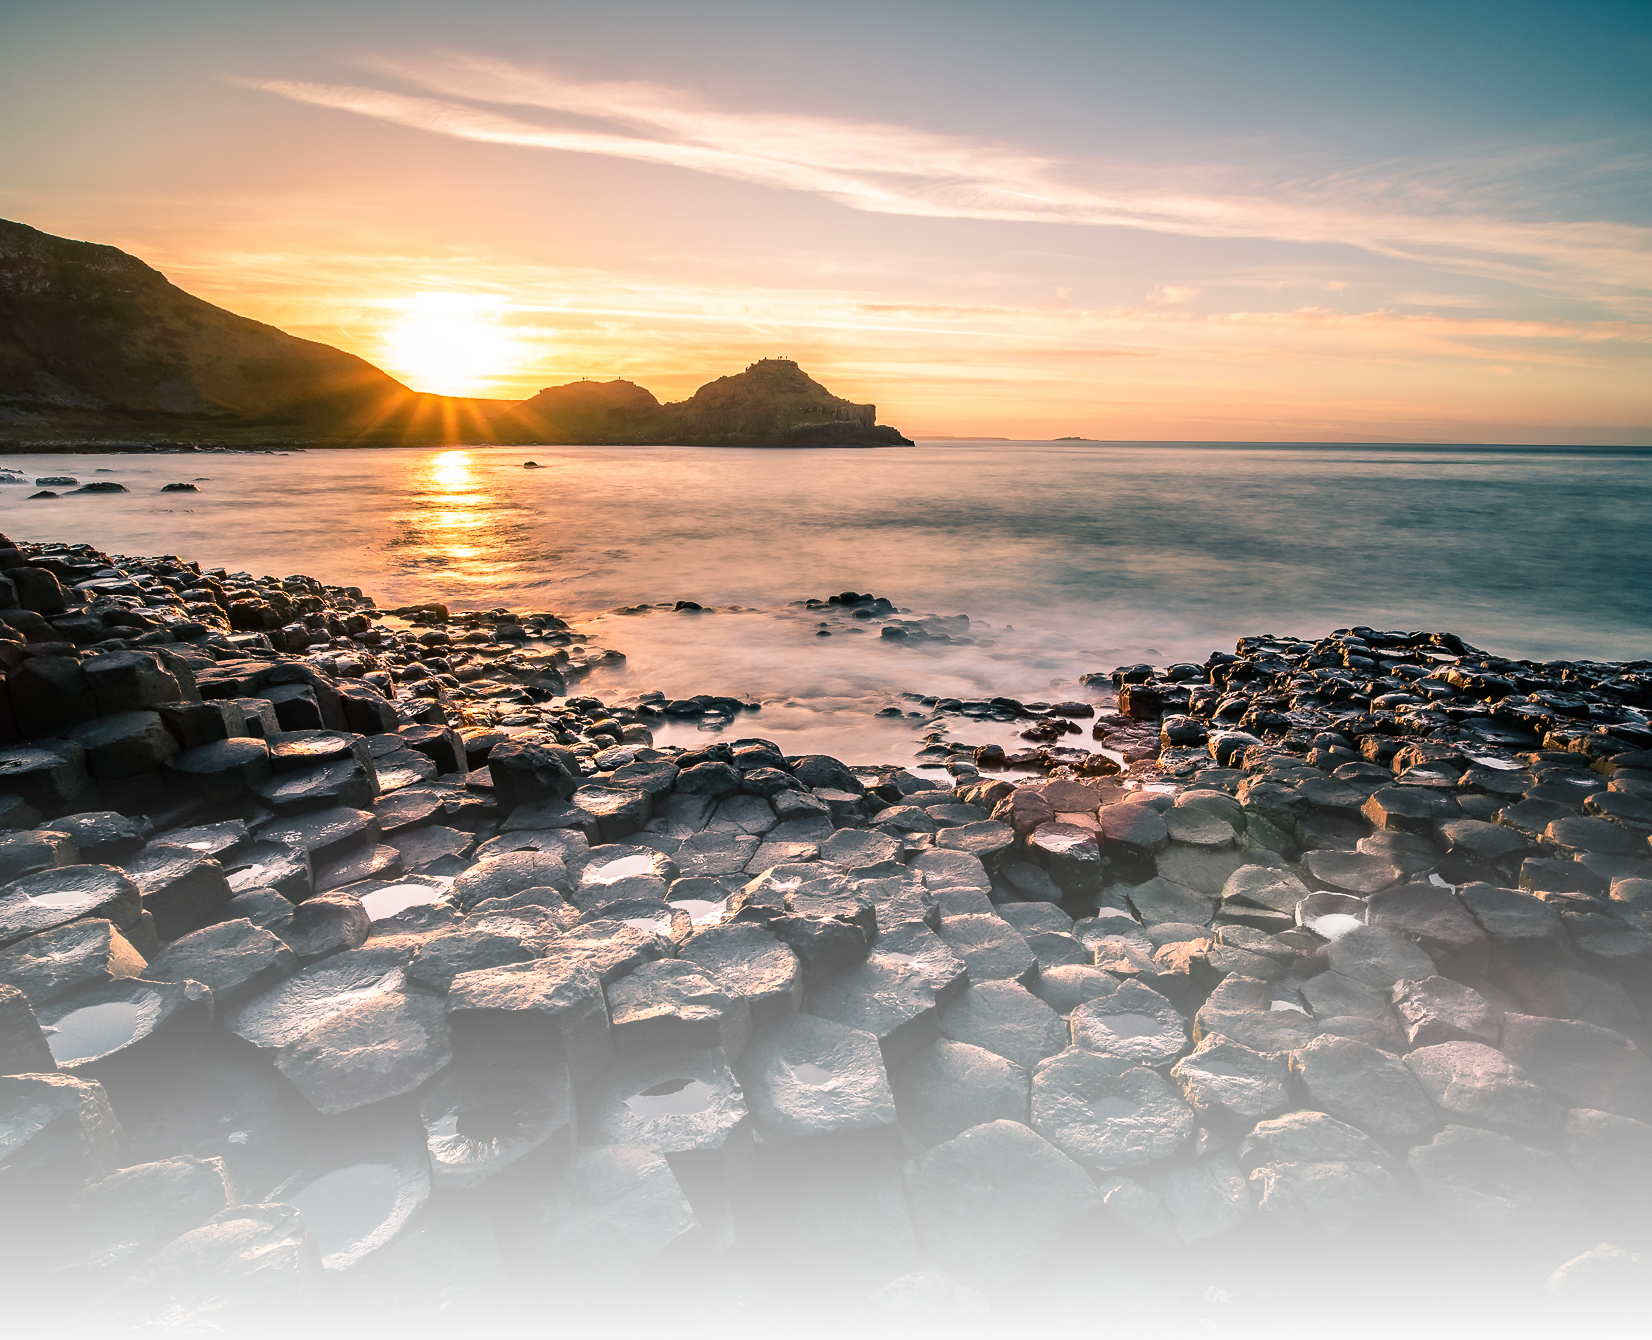
\includegraphics[width=\paperwidth]{hexagons2}}
};
\end{tikzpicture}
%\vfill
\vspace{1cm}

\textcolor{white}{
%\begin{flushleft}
\titlefont Differential Cohomology \\[0.3cm]
\subtitlefont Categories, Characteristic\\Classes, and Connections\\[0.75cm]
\subsubtitlefont Edited by Araminta Amabel, Arun Debray, and Peter Haine
%\end{flushleft}
}
\end{center}
